\documentclass{article}
\usepackage{mathtools}
\begin{document}
	\section*{Lsg Vorschlag LAÜ07 Maximilian Maag}
	\section*{Aufgabe A}
	\begin{itemize}
		\item richtig
		\item falsch
		\item richtig
		\item richtig
		\item falsch
	\end{itemize}
	\section*{Aufgabe B}
	\section*{Aufgabe 1}
	Universeller Ansatz, wenn LGS Matrix invertierbar: $\vec{x}$ = $A^{-1} \cdot \vec{b}$
	\subsection*{a)}
	A = 
	$\left(\begin{array}{ccc}
	 1 & 0 & 1 \\ -2 & 5 & -4 \\ 5 & 8 & 2
	\end{array}\right)$
	$\vec{b}$ =
	$\left(\begin{array}{c}
	1 \\ 1 \\ 12
	\end{array}\right)$ \\ \\
	$A^{-1}$ =
	$\left(\begin{matrix}
		42 & 8 & -5 \\
		-16 & -3 & 2 \\
		-41 & -8 & 5
	\end{matrix}\right)
    $ \\
    $\vec{x}$ = 
    $\left(\begin{matrix}
    42 & 8 & -5 \\
    -16 & -3 & 2 \\
    -41 & -8 & 5
    \end{matrix}\right) $
    $\cdot$
    $\left(\begin{array}{c}
    1 \\ 1 \\ 12
    \end{array}\right)$ \\
    $\left(\begin{array}{c}
    x \\ y \\ z
    \end{array}\right)$ =
     $\left(\begin{matrix}
    42 & 8 & -5 \\
    -16 & -3 & 2 \\
    -41 & -8 & 5
    \end{matrix}\right) $
    $\cdot$
    $\left(\begin{array}{c}
    1 \\ 1 \\ 12
    \end{array}\right)$ \\
     $\left(\begin{array}{c}
    x \\ y \\ z
    \end{array}\right)$
    = 
   $ \left(\begin{matrix}
    	-10 \\
    	5 \\
    	11
    \end{matrix}\right)$ \\ \\
    x = -10; y = 5; z = 11
	\subsection*{b)}
	A = 
	$\left(\begin{array}{ccc}
	2 & 1 & 1 \\ 0 & 3 & -1 \\ 5 & 5 & 2
	\end{array}\right)$
	$\vec{b}$ =
	$\left(\begin{array}{c}
	1 \\ 2 \\ 3 
	\end{array}\right)$ \\
	$A^{-1}$ =
	$
	\left(\begin{matrix}
	\frac{11}{2} & \frac{3}{2} & -2 \\
	\frac{-5}{2} & \frac{-1}{2} & 1 \\
	\frac{-15}{2} & \frac{-5}{2} & 3
	\end{matrix}\right)
	$ \\
	$\vec{x}$ = 
	$
	\left(\begin{matrix}
	\frac{11}{2} & \frac{3}{2} & -2 \\
	\frac{-5}{2} & \frac{-1}{2} & 1 \\
	\frac{-15}{2} & \frac{-5}{2} & 3
	\end{matrix}\right)
	$  $\cdot$
	$
	\left(\begin{array}{c}
		1 \\ 2 \\ 3 
	\end{array}\right)
	$ \\
	$
	\left(\begin{array}{c}
	x \\ y  \\ z
	\end{array}\right)
	$ =
	$
	\left(\begin{matrix}
	\frac{5}{2} \\
	\frac{-1}{2} \\
	\frac{-7}{2}
	\end{matrix}\right)
	$ \\ \\
	x = $\frac{5}{2}$ \\
	y = $-\frac{1}{2}$ \\
	z = $-\frac{7}{2}$
	
	\section*{Aufgabe 2}
	\subsection*{a)}
	A = 
	$\left(\begin{array}{ccc}
	 \frac{8}{10} & \frac{1}{10} & \frac{1}{10} \\ \frac{2}{10} & \frac{6}{10} & \frac{2}{10} \\ \frac{2}{10} & \frac{2}{10} &\frac{6}{10}
	\end{array}\right)$
	\subsection*{b)}
	Aktuell: \\
	$\vec{b_{0}}$ = 
	$
	\left(\begin{array}{c}
	\frac{4}{10} \\ \frac{4}{10} \\ \frac{2}{10} 
	\end{array}\right)
	$ \\
	1 Jahr später: \\
	$\vec{b_{1}}$ = A $\cdot$ $\vec{b_{0}}$ \\
	$\vec{b_{1}}$ =
	$\left(\begin{array}{ccc}
	\frac{8}{10} & \frac{1}{10} & \frac{1}{10} \\ \frac{2}{10} & \frac{6}{10} & \frac{2}{10} \\ \frac{2}{10} & \frac{2}{10} &\frac{6}{10}
	\end{array}\right)$ 
	$\cdot$
	$
	\left(\begin{array}{c}
	\frac{4}{10} \\ \frac{4}{10} \\ \frac{2}{10} 
	\end{array}\right)
	$ \\
	$\vec{b_{1}}$ =
	$\left(\begin{array}{c}
	 \frac{38}{100} \\ \frac{36}{100} \\ \frac{28}{100}
	\end{array}\right)$ \\ \\
	Standort A: 38 Prozent \\
	Standort B: 36 Prozent \\
	Standort C: 28 Prozent \\ \\
	Vollständige Multiplikation in Material 1. \\
	Nach 2 Jahren: \\
	$\vec{b_{2}}$ = A $\cdot$ $\vec{b_{1}}$ \\
	$\vec{b_{2}}$ =
	$\left(\begin{array}{ccc}
	\frac{8}{10} & \frac{1}{10} & \frac{1}{10} \\ \frac{2}{10} & \frac{6}{10} & \frac{2}{10} \\ \frac{2}{10} & \frac{2}{10} &\frac{6}{10}
	\end{array}\right)$ 
	$\cdot$
	$\left(\begin{array}{c}
	\frac{38}{100} \\ \frac{36}{100} \\ \frac{28}{100}
	\end{array}\right)$ \\
	$\vec{b_{2}}$ = 
	$
	\left(\begin{matrix}
	\frac{4}{5}*\left(\frac{19}{50}\right)+\frac{1}{10}*\left(\frac{9}{25}\right)+\frac{1}{10}*\left(\frac{7}{25}\right) \\
	\frac{1}{5}*\left(\frac{19}{50}\right)+\frac{3}{5}*\left(\frac{9}{25}\right)+\frac{1}{5}*\left(\frac{7}{25}\right) \\
	\frac{1}{5}*\left(\frac{19}{50}\right)+\frac{1}{5}*\left(\frac{9}{25}\right)+\frac{3}{5}*\left(\frac{7}{25}\right)
	\end{matrix}\right)
	$ \\
	$\vec{b_{2}}$ = 
	$
	\left(\begin{matrix}
	\frac{46}{125} \\
	\frac{87}{250} \\
	\frac{79}{250}
	\end{matrix}\right)
	$ \\ \\
	A: 0,368 $\approx$ 36,8 Prozent \\
	B: 0,348 $\approx$ 34,8 Prozent \\
	C: 0,316 $\approx$ 31,6 Prozent
	\subsection*{c)}
	Ansatz in Material 3. \\ \\
	A = 
	$\left(\begin{array}{ccc}
	\frac{8}{10} & \frac{1}{10} & \frac{1}{10} \\ \frac{2}{10} & \frac{6}{10} & \frac{2}{10} \\ \frac{2}{10} & \frac{2}{10} &\frac{6}{10}
	\end{array}\right)$ 
	$A^{-1}$ = 
	$
	\left(\begin{matrix}
		\frac{4}{3} & \frac{-1}{6} & \frac{-1}{6} \\
		\frac{-1}{3} & \frac{23}{12} & \frac{-7}{12} \\
		\frac{-1}{3} & \frac{-7}{12} & \frac{23}{12}
	\end{matrix}\right)
	$ \\
	$\vec{b_{-1}}$ = 
	$
	\left(\begin{matrix}
	\frac{4}{3} & \frac{-1}{6} & \frac{-1}{6} \\
	\frac{-1}{3} & \frac{23}{12} & \frac{-7}{12} \\
	\frac{-1}{3} & \frac{-7}{12} & \frac{23}{12}
	\end{matrix}\right)
	$
	$\cdot$
	$
	\left(\begin{array}{c}
	\frac{4}{10} \\ \frac{4}{10} \\ \frac{2}{10} 
	\end{array}\right)
	$ \\
	$\vec{b_{-1}}$ =
	$
	\left(\begin{matrix}
	\frac{4}{3}*\left(\frac{2}{5}\right)+\frac{-1}{6}*\left(\frac{2}{5}\right)+\frac{-1}{6}*\left(\frac{1}{5}\right) \\
	\frac{-1}{3}*\left(\frac{2}{5}\right)+\frac{23}{12}*\left(\frac{2}{5}\right)+\frac{-7}{12}*\left(\frac{1}{5}\right) \\
	\frac{-1}{3}*\left(\frac{2}{5}\right)+\frac{-7}{12}*\left(\frac{2}{5}\right)+\frac{23}{12}*\left(\frac{1}{5}\right)
	\end{matrix}\right)
	$ \\
	$\vec{b_{-1}}$ =
	$
	\left(\begin{matrix}
	\frac{13}{30} \\
	\frac{31}{60} \\
	\frac{1}{60}
	\end{matrix}\right)
	$ \\ \\
	A: 0,433333... $\approx$ 43,33 Prozent \\
	B: 0,51666... $\approx$ 51,66 Prozent \\
	C: 0,016666... $\approx$ 1,66 Prozent
	\subsection*{d)}
	Ansatz in Material 4. \\ \\
	A $\cdot$ $\vec{x}$ = $\vec{x}$ \\ \\
	$\left(\begin{array}{ccc}
	\frac{8}{10} & \frac{1}{10} & \frac{1}{10} \\ \frac{2}{10} & \frac{6}{10} & \frac{2}{10} \\ \frac{2}{10} & \frac{2}{10} &\frac{6}{10}
	\end{array}\right)$ $\cdot$
	$\left(\begin{array}{c}
	x \\ y \\ z
	\end{array}\right)$
	= 
	$\left(\begin{array}{c}
	x \\ y \\ z
	\end{array}\right)$ \\ \\
	$\begin{array}{ccc}
	\frac{8}{10}x & \frac{1}{10}y & \frac{1}{10}z \\ \frac{2}{10}x & \frac{6}{10}y & \frac{2}{10}z \\ \frac{2}{10}x & \frac{2}{10}y &\frac{6}{10}z
	\end{array}$
	$\begin{array}{c}
		= \\ = \\ = 
	\end{array}$
	$\begin{array}{c}
	x \\ y \\ z
	\end{array}$ \\ \\
	$\begin{array}{ccc}
	-\frac{2}{10}x & \frac{1}{10}y & \frac{1}{10}z \\ \frac{2}{10}x & -\frac{4}{10}y & \frac{2}{10}z \\ \frac{2}{10}x & \frac{2}{10}y &-\frac{4}{10}z
	\end{array}$
	$\begin{array}{c}
	= \\ = \\ = 
	\end{array}$
	$\begin{array}{c}
	0 \\ 0 \\ 0
	\end{array}$ \\ \\
	$\begin{array}{ccc}
	-2x & 1y & 1z \\ 2x & -4y & 2z \\ 2x & 2y &-4z
	\end{array}$
	$\begin{array}{c}
	= \\ = \\ = 
	\end{array}$
	$\begin{array}{c}
	0 \\ 0 \\ 0
	\end{array}$ \\
	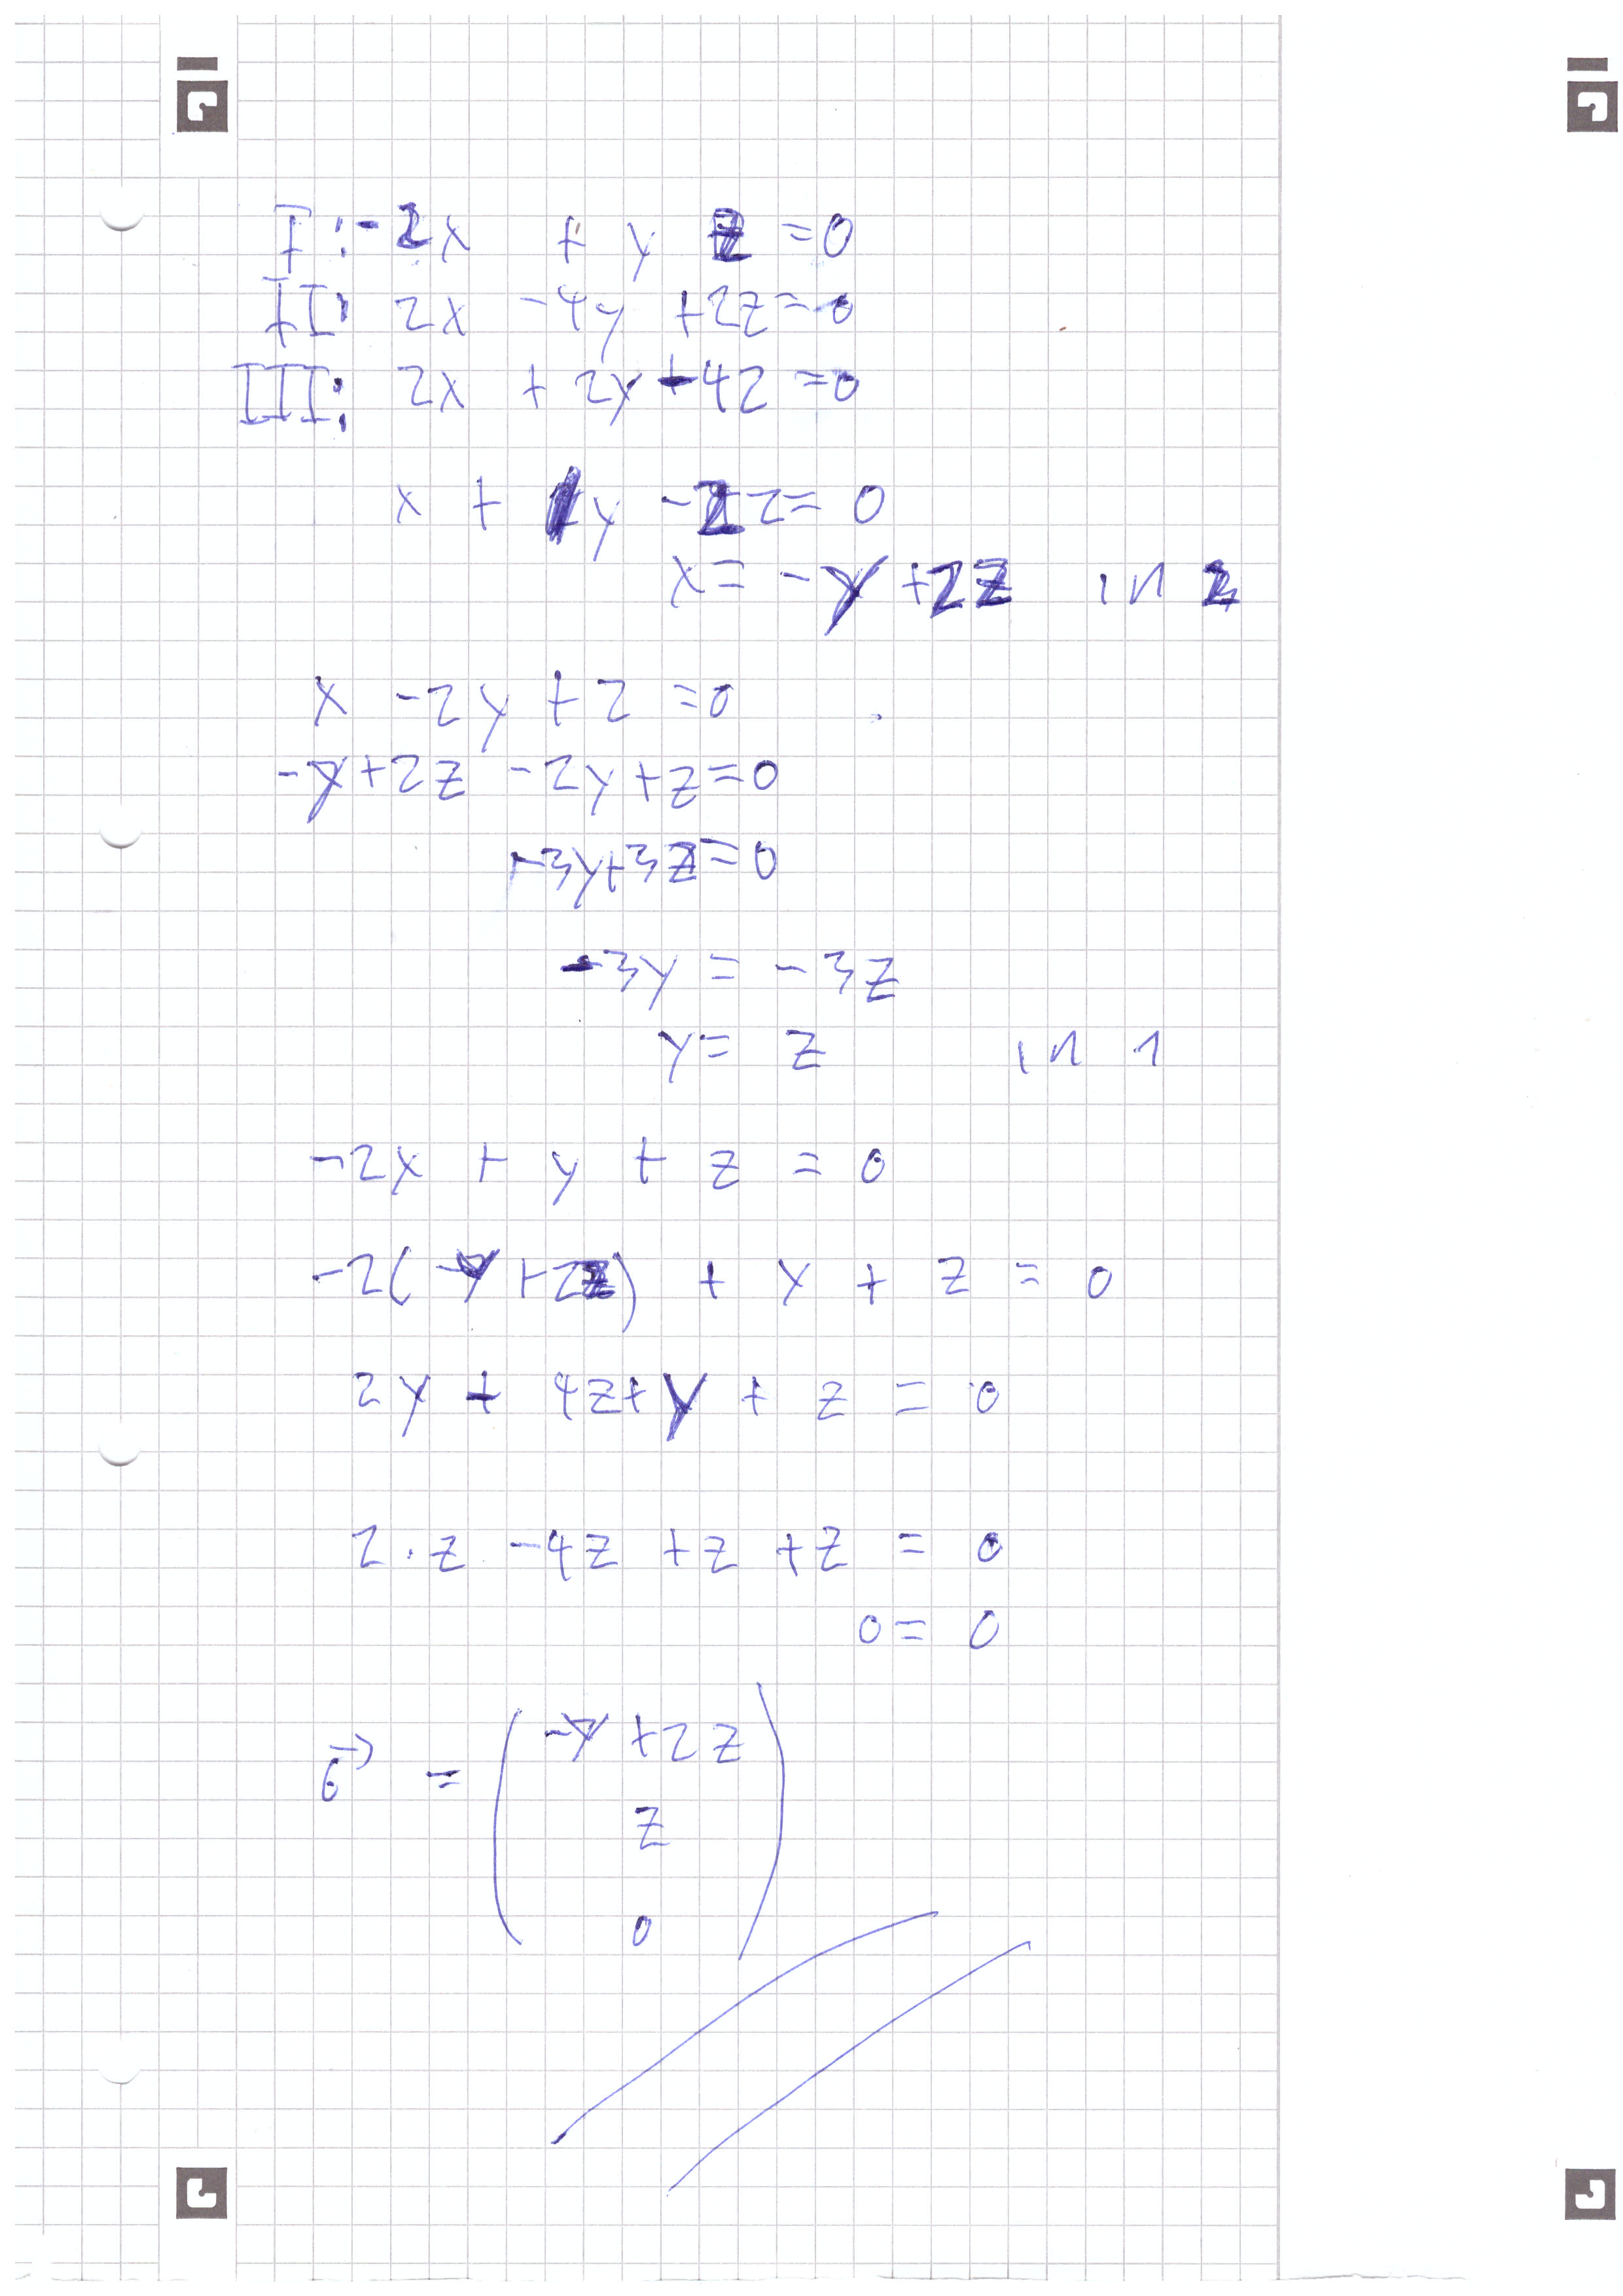
\includegraphics[width=\linewidth]{072d1}
	\section*{Aufgabe 3}
	Es sei A und B je eine n x n Matrix, für die Invertierbarkeit gelte. \\
	\\
	Zu Zeigen: $(A \cdot B)^{-1} = B^{-1} \cdot A^{-1}$ \\ \\
	$(AB)^{-1}  \cdot AB =  B^{-1}A^{-1} \cdot AB$ \\
	$E =  B^{-1}(A^{-1} \cdot A)B$ \\
	$E =  B^{-1} \cdot E \cdot B$ \\
	$E =  B^{-1} \cdot B $ \\
	$E =  E $ \\
	q.e.d. \\ \\
	Die Idee zu diesem Beweis befindet sich in Material 2.
	\section*{Material}
	In dieser Sektion sind meine handschriftlichen Nebenrechnungen, Überlegungen, Notizen und Kritzeleien.
	\subsection*{Material 1}
	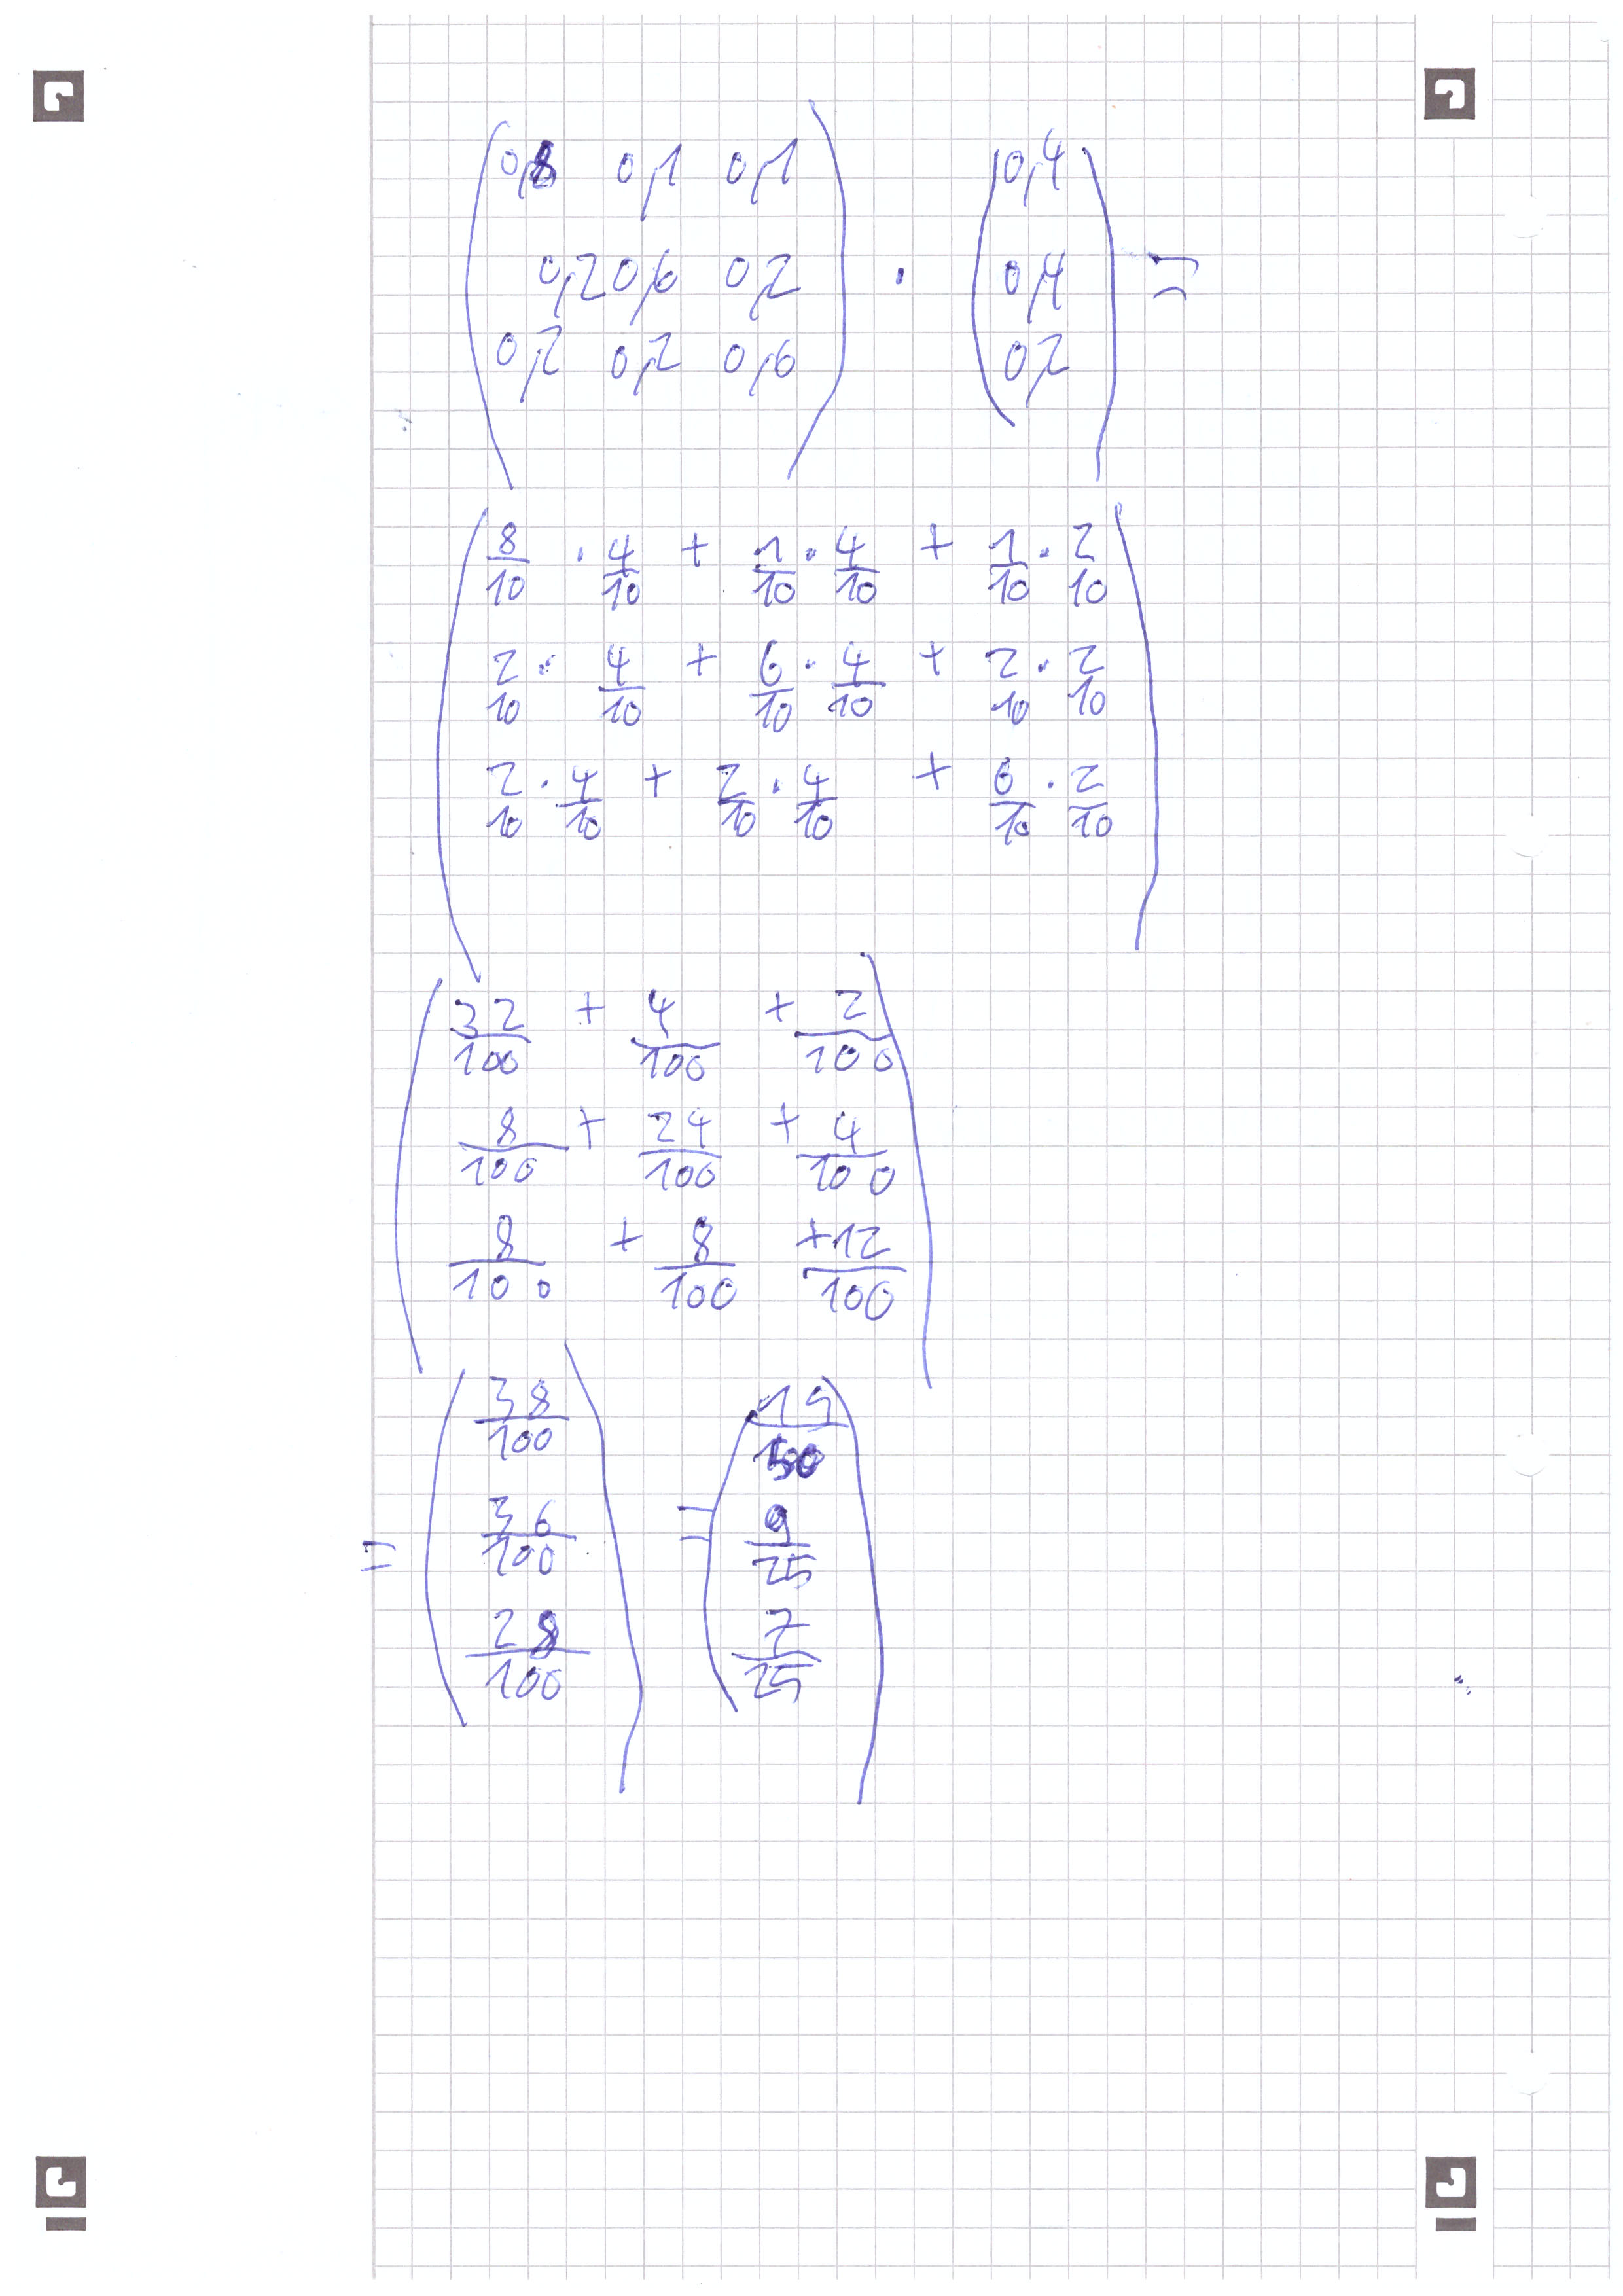
\includegraphics[width=\linewidth]{0702b.png}
	\subsection*{Material 2}
	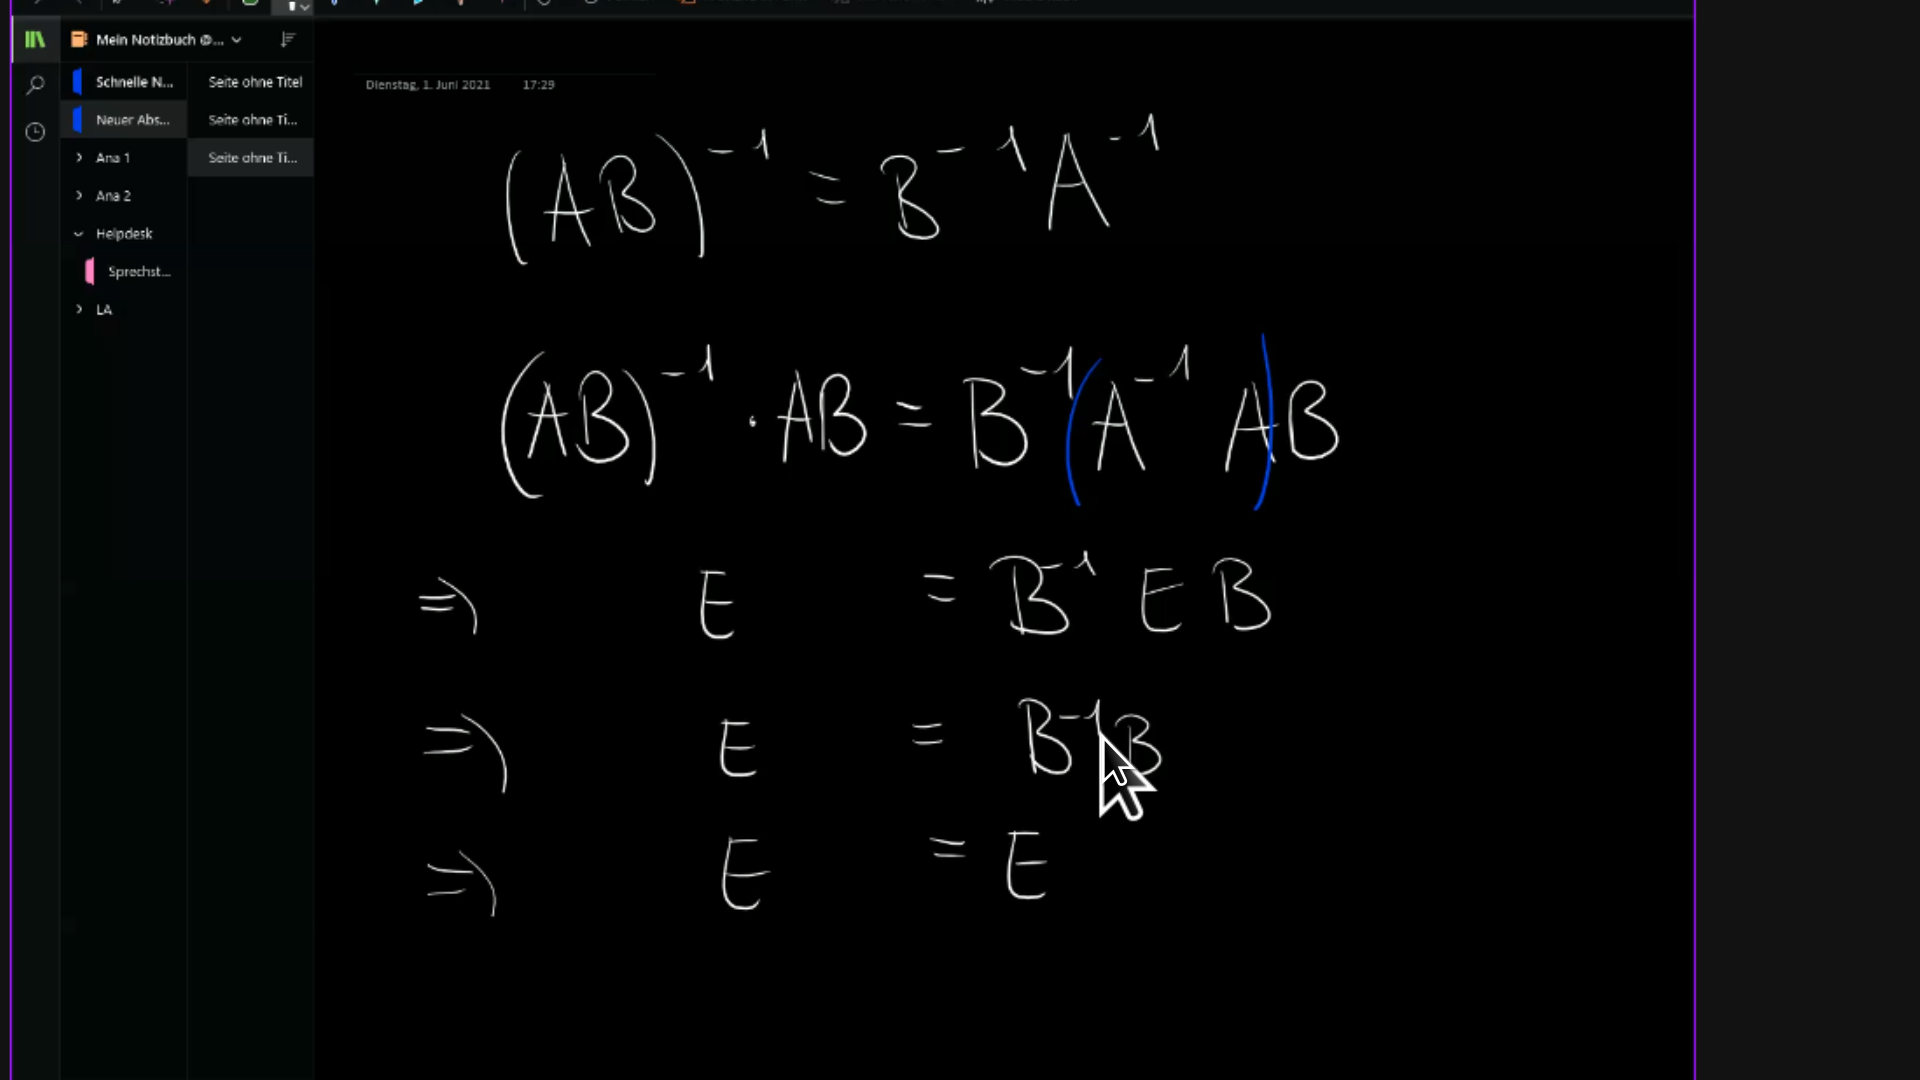
\includegraphics[width=\linewidth]{0703} \\
	Idee für den Beweis aus Aufgabe 3. Man kann sich überlegen was allgemein für eine Einheitsmatrix gilt und durch was man diese Ersetzen könnte.
	\subsection*{Material 3}
	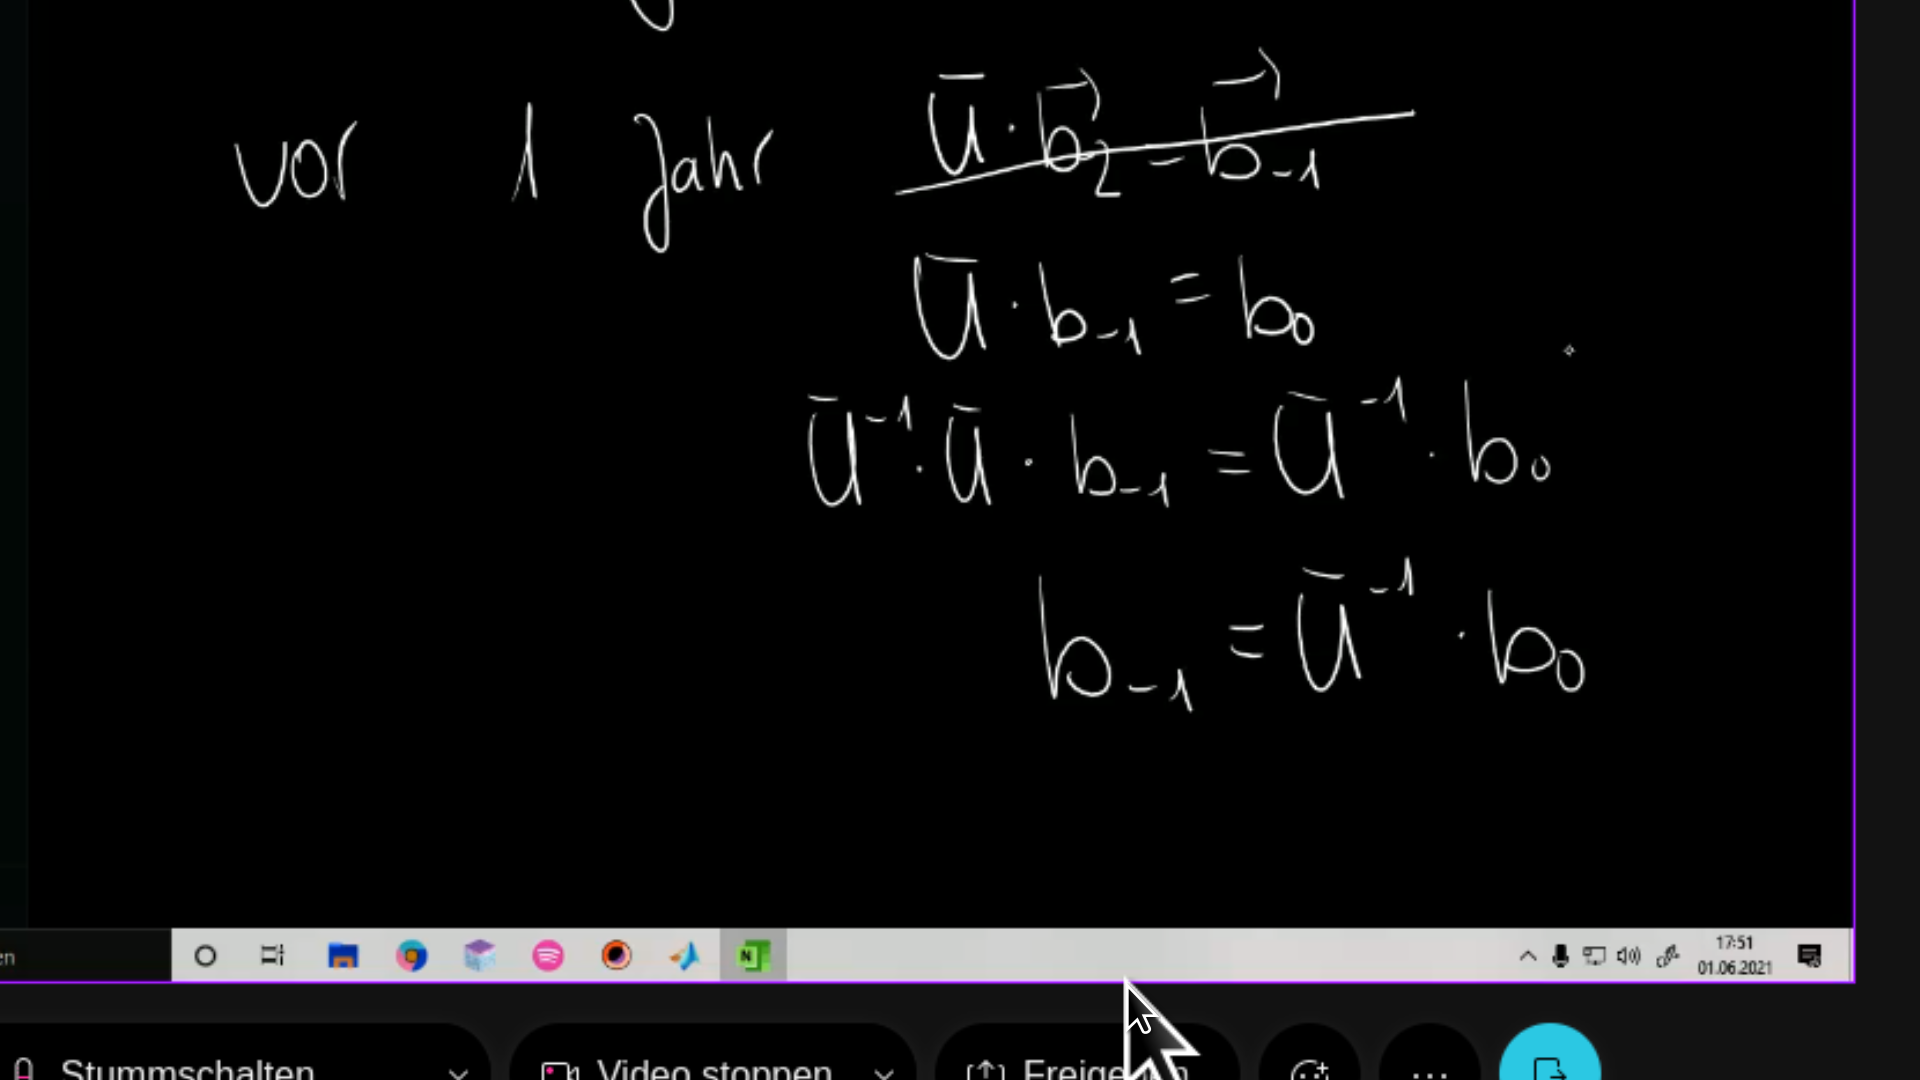
\includegraphics[width=\linewidth]{072c} \\
	Die Belegung rückwirkend zu berechnen ist schwierig. Mit der Inversen und dem Ausgangsstatus ist jedoch möglich.
	\subsection*{Material 4}
	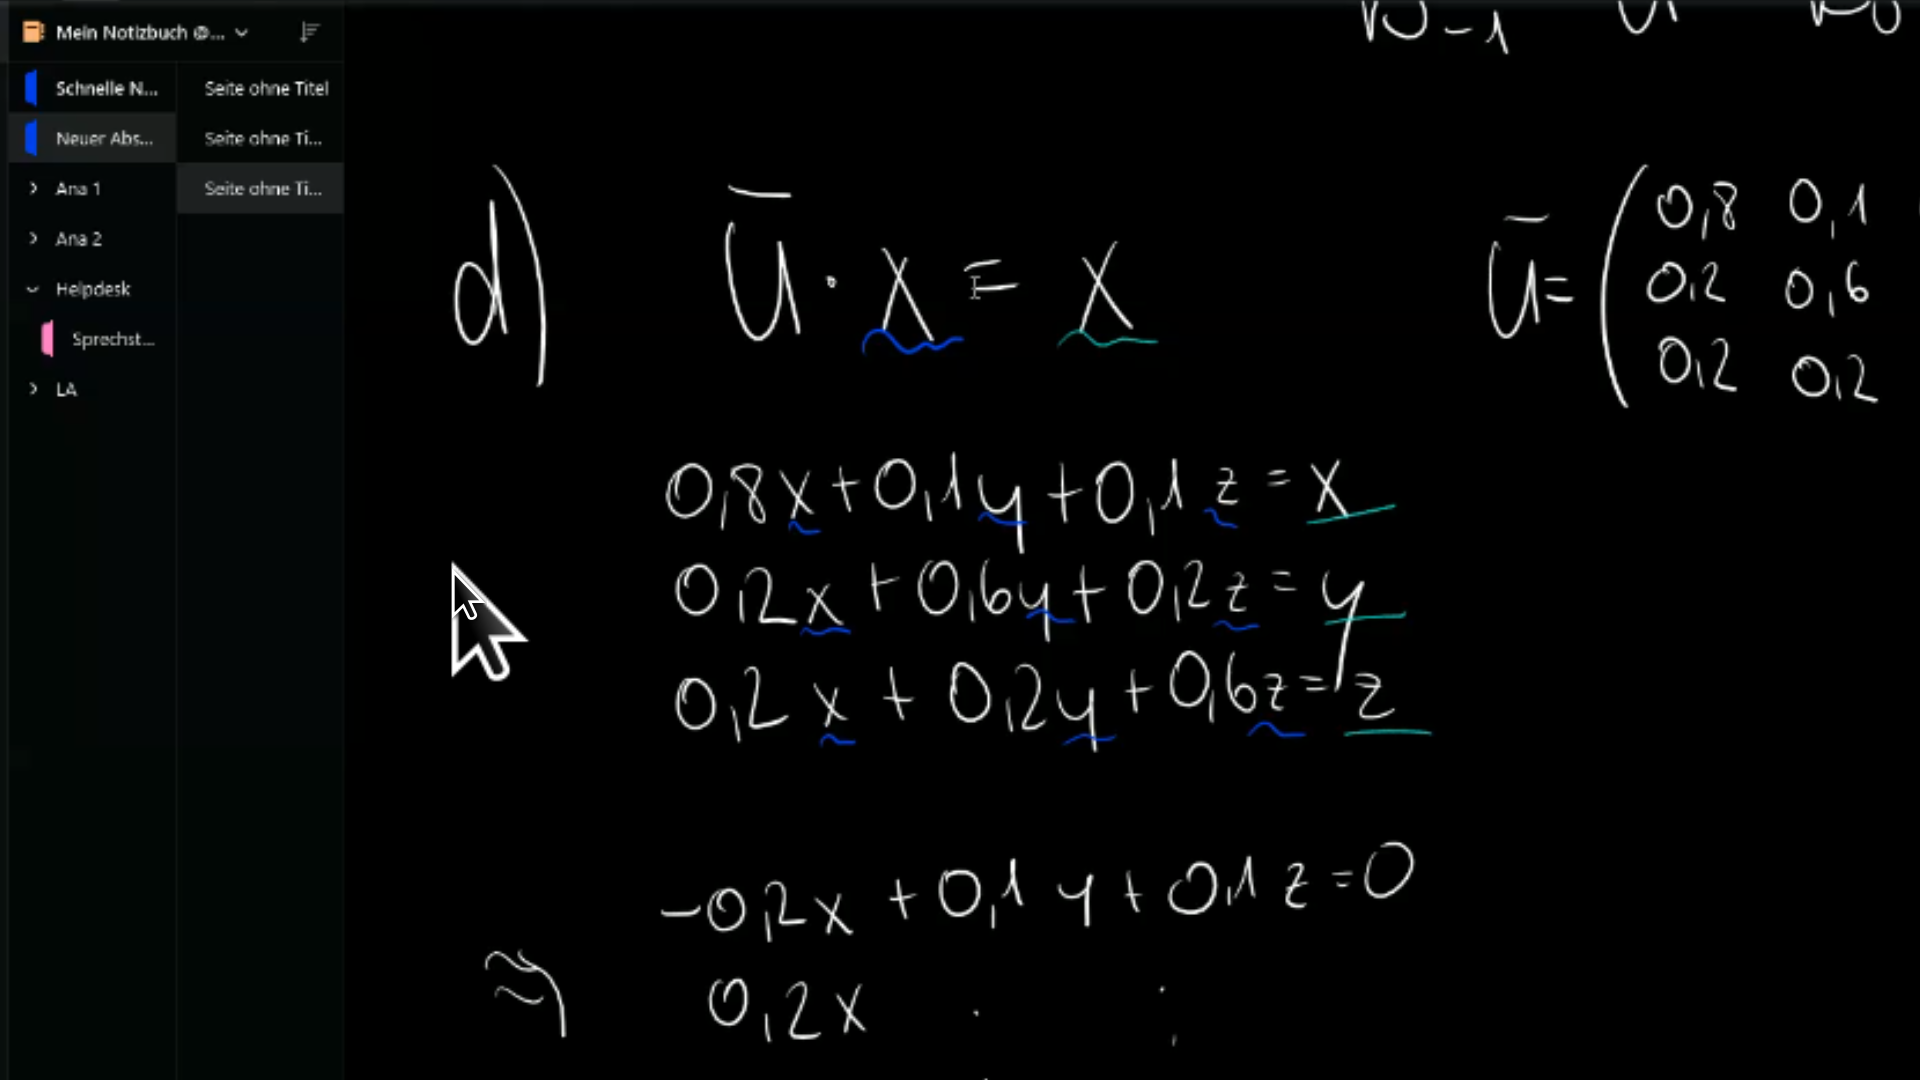
\includegraphics[width=\linewidth]{072d} \\
	Das LGS hat zwar die triviale Lösung: \\
	$\left(\begin{array}{c}
	0 \\ 0 \\ 0
	\end{array}\right)$ \\
	Allerdings sind hier Abhängigkeiten gefordert um allgemein zu beschreiben mit welchem Vektor sich die Verteilung stabilisiert (glaube ich zumindest).
\end{document}